% !TeX root = Protokoll.tex

\begin{figure}[h!]
	\centering
	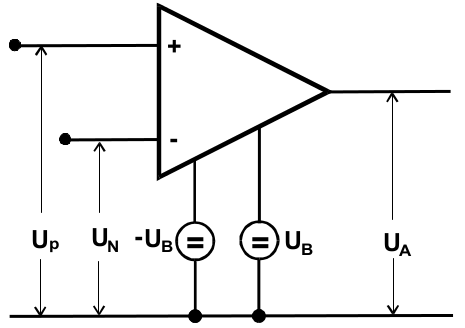
\includegraphics[width= 0.5\textwidth]{../Grafiken/OP_Schaltung.png}
	\caption{Hier ist die skizzierte Schaltung eines Operationsverstärkers dargestellt. \cite{V51}\label{fig:OP_Schaltung}}
\end{figure}
In \cref{fig:OP_Schaltung} ist die Schaltung für einen Operationsverstärker dargestellt.
Ein Operationsverstärker wird durch zwei konstante Betriebsspannungen $U_\text{B}$ und $-U_\text{B}$ betrieben.
Weiter ist die resultierende Ausgangsspannung $U_\text{A}$ als
\begin{align}
	U_\text{A}=V(U_\text{P}-U_\text{N})
\end{align}
gegeben. 
Dabei ist $U_P$ die Spannung des nicht-invertierenden Eingangs, $U_N$ die Spannung des invertierenden Eingangs und $V$ ist die Leerlaufverstärkung.
Dabei wird die Spannung verstärkt, wenn 
\begin{align*}
	-U_\text{B}<U_\text{A}<U_\text{B}
\end{align*}
außerhalb dieses Intervalls ist die Ausgangsspannung $U_\text{A}=\pm U_\text{B}$.
Die Kennlinie ist in \cref{fig:Kennlinie} dargestellt.
\begin{figure}
	\centering
	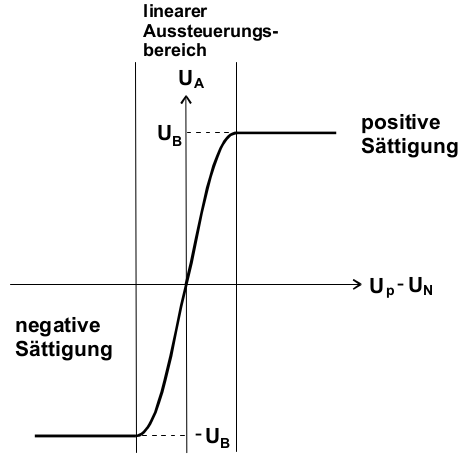
\includegraphics[width = 0.5\textwidth]{../Grafiken/Op_Kennlinie.png}
	\caption{Hier ist die Kennlinie eines Operationsverstärkers Dargestell. \cite{V51}\label{fig:Kennlinie}}
\end{figure} 
Ein  Operationsverstärker wird, neben der Leerlaufverstärkung $V$, durch mehrere Komponenten beschrieben.
Den beiden Eingangswiederständen $r_{\text{e}_{{}_\text{P}}}$ und $r_{\text{e}_{{}_\text{N}}}$ sowie den Ausgangswiederstand $r_\text{a}$.
Die Leerlaufverstärkung $V$ ist im allgemeinen Fall sehr groß und abhängig von der Frequenz, weswegen sie für einen idealen Operationsverstärker als unendlich angenommen wird.
Die Eingangswiderstände sind sehr groß, weswegen die idealen als unendlich angenommen werden.
Der Ausgangswiederstand hingegen ist klein, weshalb der ideale als null angenommen werden kann.
\begin{align}
	V_\text{id}=\infty,~ r_{\text{e}_\text{id}}=\infty,~ r_{\text{a}_\text{id}}=0
\end{align}
Für einen realen Operationsverstärker müssen weitere Kenngrößen eingeführt werden.
Aufgrund von Asymmetrien in einem realen Operationsverstärker ist die Ausgangsspannung ungleich null, auch wenn zwei gleiche Spannungen an den Eingängen angelegt werden.
Deshalb ist es hilfreich die Gleichtaktverstärkung zu definieren $V_\text{Gl}$
\begin{align}
	V_\text{Gl}:=\frac{\Delta U_\text{A}}{\Delta U_\text{Gl}}.
\end{align}
Weiter treten Eingangsströme $I_\text{N}$ und $I_\text{P}$ auf, aufgrund der endlichen Eingangswiederstände in einem realen Operationsverstärkers.
Daraus lässt sich der Ruhestrom $I_\text{B}$ definieren als
\begin{align}
	I_\text{B}:=\frac{1}{2}\left( I_\text{P} + I_\text{N} \right)
\end{align}
